\documentclass[fleqn]{homework}

\student{Stephen Brennan (smb196)}
\course{EECS 477}
\assignment{Homework 3}
\duedate{October 11, 2015}

\usepackage{enumerate}
\usepackage{mathtools}
%\usepackage{graphicx}

\begin{document}
  \maketitle

  \begin{problem}{1}
    \begin{question}
      Consider the minimum cost network flow problem defined on the following
      network $G=(V, E)$. The node set $V$ consists of the six nodes $a$, $b$,
      $c$, $d$, $e$, and $f$. Each node has a capacity, which is defined as the
      maximum amount of flow that can cross that node. The nodes have supplies
      and capacities as per the following table:

      \begin{tabular}{|r|r|r|}
        \hline
        Node & $b_i$ & capacity \\
        \hline
        $a$ & 20 & 25 \\
        $b$ & 5 & 35 \\
        $c$ & -15 & 30 \\
        $d$ & -10 & 10 \\
        $e$ & 0 & 20 \\
        \hline
      \end{tabular}

      The network has six arcs, whose costs, lower bounds, and upper bounds are
      as follows:

      \begin{tabular}{|l|r|r|r|}
        \hline
        Arc & $c$ & $l$ & $u$ \\
        $(a,b)$ & 4 & 5 & $\infty$ \\
        $(a,c)$ & 6 & 3 & $\infty$ \\
        $(b,c)$ & -2 & 0 & 25 \\
        $(b,e)$ & 5 & 0 & 10 \\
        $(c,d)$ & -3 & 5 & 10 \\
        $(e,d)$ & 2 & 0 & $\infty$ \\
        \hline
      \end{tabular}

      \begin{enumerate}[a.]
      \item Draw an equivalent minimum cost network flow problem on a network in
        which nodes have no capacities, arc lower bounds are zero, arc upper
        bounds are infinity, and costs are positive.

      \item Show that the following flow is feasible, and draw the corresponding
        residual network:
      \end{enumerate}

      \begin{tabular}{|l|r|}
        \hline
        Arc & Flow \\
        \hline
        $(a,b)$ & 20 \\
        $(a,c)$ & 0 \\
        $(b,c)$ & 25 \\
        $(b,e)$ & 0 \\
        $(c,d)$ & 10 \\
        $(e,d)$ & 0 \\
        \hline
      \end{tabular}
    \end{question}
  \end{problem}

  \begin{problem}{2}
    \begin{question}
      Give an example of a minimum cost network flow problem in which there is
      an optimal solution that is fractional.
    \end{question}
  \end{problem}

  \begin{problem}{3}
    \begin{question}
      Consider the minimum cost network flow problem in problem 1.  Write the
      dual and the complementary slackness conditions.  For simplicity, you are
      allowed to transform the problem into an equivalent one from which the
      dual can be more easily derived.
    \end{question}
  \end{problem}

  \begin{problem}{4}
    \begin{question}
      Consider the minimum cost network flow problem defined on the following
      graph:

      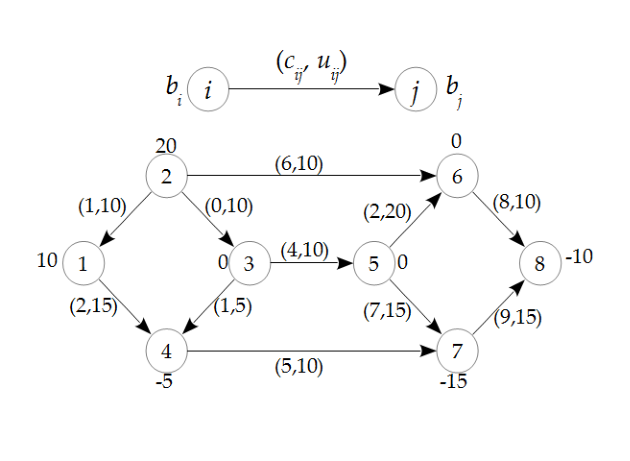
\includegraphics{problem4-network.pdf}

      An optimal solution $x^*$ is:

      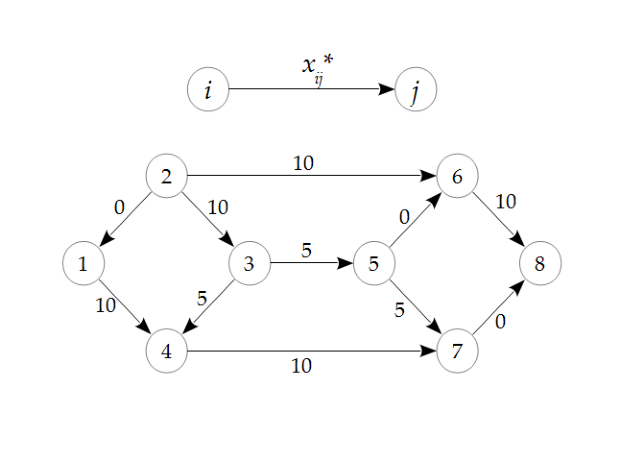
\includegraphics{problem4-flow.pdf}

      In this instance of minimum cost network flow:
      \begin{enumerate}[a.]
        \item Draw the residual network $G(x^*)$.
        \item Specify a set of node potentials $\pi$ that together with $x^*$
          satisfy the reduced cost optimality conditions.  List each arc in the
          residual network and its reduced cost.
        \item Verify that the solution $x^*$ satisfies the complementary
          slackness optimality conditions.  To do so, specify a set of node
          potentials and list the reduced cost of each arc.
      \end{enumerate}
    \end{question}
  \end{problem}

  \begin{problem}{5}
    \begin{question}
      Two players, called Alice and Bob, play the following game. A set of
      gambling chips are placed on a line. Gambling chips can have arbitrary
      integer values. Then, the players take turn removing one of the chips from
      either end of the remaining line of chips. In other words, at his turn,
      each player removes the chip either at the left or at the right end of the
      line (his choice, but not in the middle) and places it in his collection.
      The player with the larger total value wins.

      \begin{enumerate}[a.]
      \item Show an arrangement of gambling chips where Alice would lose if she
        always picked the end-of-line chip with the largest possible value.
      \item Design an algorithm that takes as input a linear arrangement of
        chips and that returns Alice’s best strategy assuming that Bob will make
        the most of the remaining chip arrangement. Your algorithm should
        formulate the game as a shortest path problem.  
      \item Determine the running time of your algorithm assuming that shortest
        paths are computed with Dijkstra’s algorithm. Suggest an improvement to
        the shortest path computation that results in a faster run time.
      \end{enumerate}
    \end{question}
  \end{problem}

  \begin{problem}{7}
    \begin{question}
      Consider problem 5 in Homework Assignment 2. Show that the linear program
      is equivalent to a minimum cost network flow problem and prove that this
      program has always an integer optimal solution.

      \textbf{Problem 5 from Homework Assignment 2:}

      \begin{align*}
        \min x_1 + x_2 + 3x_3 + 2x_4 + 4x_5 & \\
        \text{s.t. } x_1 + x_3 + x_5 &= 2 \\
        x_4 - x_3 &= 1 \\
        x_2 - x_1 &= -1 \\
        x_2 + x_4 + x_5 &= 2 \\
        0 \le x_1 &\le 1 \\
        0 \le x_2 &\le 2 \\
        0 \le x_3 &\le 1 \\
        0 \le x_4 &\le 3 \\
        0 \le x_5 &\le 2 \\
      \end{align*}
    \end{question}
  \end{problem}

\end{document}